%//==============================--@--==============================//%

A maior parte da energia elétrica que consumimos provém de \textit{geradores síncronos} ou \textit{alternadores trifásicos}, fundamentais nos Sistemas de Energia Elétrica. Estas máquinas transformam energia mecânica em elétrica através da lei da indução eletromagnética de Faraday (conversores mecanoelétricos).

O termo \textit{síncrona} refere-se à capacidade destas máquinas operarem a uma velocidade e frequência constantes, em sintonia com outras ligadas à mesma rede. Na prática, um gerador pode receber energia mecânica de várias fontes, como turbinas hidráulicas ou a vapor, e converter essa energia em eletricidade com eficiência elevada. Curiosamente, estas máquinas também podem funcionar como motores, absorvendo energia elétrica e fornecendo energia mecânica (funcionamento como \textit{motor síncrono}).

%//==============================--@--==============================//%
\subsection{Princípio de Funcionamento}

A máquina síncrona é constituída por uma massa metálica fixa (\textit{estator}) na qual está instalado o \textit{enrolamento induzido}, e por uma massa metálica rotativa (\textit{rotor}) no qual está bobinado o \textit{enrolamento indutor} (ou de \textit{excitação}):

O enrolamento indutor é percorrido por uma corrente contínua, que dá origem a um fluxo magnético que se fecha através do entreferro e do estator. Uma vez que o rotor, acionado pela máquina motriz, roda com velocidade constante, cria-se no entreferro um fluxo magnético girante.

O enrolamento do estator é constituído por bobinas, alojadas em cavas; as bobinas correspondente a uma fase são colocadas em cavas diretamente opostas. De acordo com a Lei de Indução, o fluxo magnético girante produz uma tensão que origina uma corrente num circuito externo ligado aos respetivos terminais. Estes enrolamentos são desfasados fisicamente por $120^{\circ}$ para que com a rotação uniforme do rotor sejam produzidas tensões desfasadas de $120^{\circ}$ no tempo, constituindo um sistema trifásico simétrico.

\vspace{0.5em}\hrule\vspace{0.5em}%

\noindent Para uma máquina com um par de pólos, a frequência da tensão induzida em ciclos por segundo (Hz) iguala a velocidade do rotor em rotações por segundo. Assim, para $50\,$Hz a velocidade de rotação deverá ser de $3000\,$ rpm. No entanto, é costume as máquinas terem mais pares de pólos (magnéticos), por exemplo 4:

\vspace{1.5em}
\noindent%
\begin{minipage}[c]{.45\linewidth}

    Cada fase é um par de enrolamentos (4 cavas): $a_1 a'_1$ e $a_2 a'_2$, $b_1 b'_1$ e $b_2 b'_2$, $c_1 c'_1$ e $c_2 c'_2$.

    \vspace{1em}
    Em cada instante são induzidas tensões iguais nos dois enrolamentos de cada fase, as quais se somam por estarem em série.

    \begin{figure}[H]
        \centering
        \includegraphics[width=.55\linewidth]{img/3/Synchronous-machine-rotor.png}
    \end{figure}
\end{minipage}\hfill
\begin{minipage}[c]{.5\linewidth}
    \centering
    \usetikzlibrary{shapes.arrows}
    \scalebox{0.5}{
    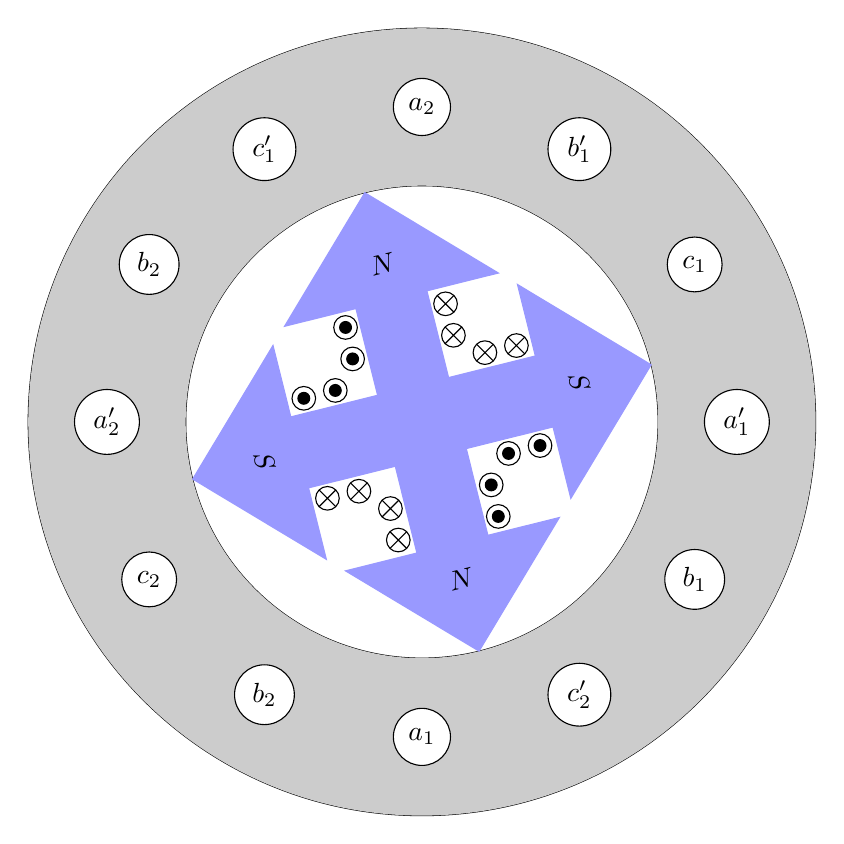
\begin{tikzpicture}[>=stealth,cross/.style={path picture={ 
    \draw[black]
    (path picture bounding box.south east) -- (path picture bounding box.north west) (path picture bounding box.south west) -- (path picture bounding box.north east);
    }}]
    
    
        % main circles
        \draw (0,0) circle (5cm);
        \draw (0,0) circle (3cm);
        \fill[gray!40,even odd rule] circle[radius=5cm] circle[radius=3cm];
        
        % small circles
        \foreach \X [count=\Y starting from 0] in {$a_2'$,$b_2$,$c_1'$,$a_2$,$b_1'$,$c_1$,$a_1'$,$b_1$,$c_2'$,$a_1$,$b_2$,$c_2$} { 
        \path(180-30*\Y:4) node[circle,draw, fill=white] (n\Y) {\X};
        }
        
        % Two-way arrow
        \node[blue!40,fill=blue!40,double arrow, draw, minimum height=6cm, minimum width=2.8cm, rotate=14,text=black] at (0,0) {};
        \node[blue!40,fill=blue!40,double arrow, draw, minimum height=6cm, minimum width=2.8cm, rotate=-76,text=black] at (0,0) {};
        
        % very small circles
        \foreach \X [count=\Y starting from 0] in {0,180} { 
            \draw[rotate around={\X:(0,0)}] (-1.5,0.3) circle (0.15cm);
            \draw[rotate around={\X:(0,0)}, fill=black] (-1.5,0.3) circle (0.075cm);
            \draw[rotate around={\X:(0,0)}] (-1.1,0.4) circle (0.15cm);
            \draw[rotate around={\X:(0,0)}, fill=black] (-1.1,0.4) circle (0.075cm);
            
            \draw[rotate around={\X:(0,0)}] (-0.97,1.2) circle (0.15cm);
            \draw[rotate around={\X:(0,0)},fill=black] (-0.97,1.2) circle (0.075cm);
            \draw[rotate around={\X:(0,0)}] (-0.88,0.8) circle (0.15cm);
            \draw[rotate around={\X:(0,0)},fill=black] (-0.88,0.8) circle (0.075cm);
        }
        
        \foreach \X [count=\Y starting from 0] in {-90,90} { 
            \draw[rotate around={\X:(0,0)}, cross] (-1.5,0.3) circle (0.15cm);
            \draw[rotate around={\X:(0,0)},cross] (-1.1,0.4) circle (0.15cm);
            
            \draw[rotate around={\X:(0,0)},cross] (-0.97,1.2) circle (0.15cm);
            \draw[rotate around={\X:(0,0)},cross] (-0.88,0.8) circle (0.15cm);
        }
        
        % Poles
        \node[rotate=14] at (-0.5,2) {$N$};
        \node[rotate=14] at (0.5,-2) {$N$};
        
        \node[rotate=-76] at (2,0.5) {$S$};
        \node[rotate=-76] at (-2,-0.5) {$S$};
    
    \end{tikzpicture}
    }
\end{minipage}

\vspace{1.5em}
\noindent Para esta situação já é necessário criar uma distinção entre o ângulo elétrico e o ângulo mecânico, de acordo com a distribuição espacial do campo magnético:

\begin{figure}[H]
    \centering
    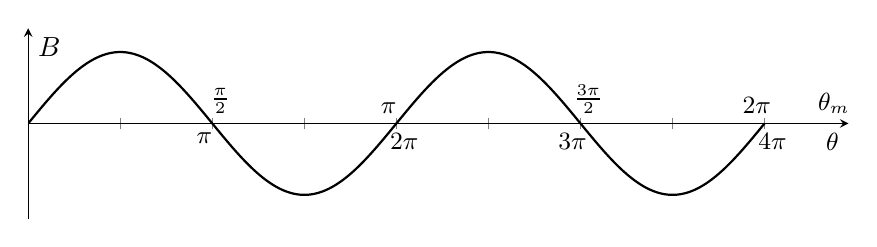
\begin{tikzpicture}
        \begin{axis}[
            xlabel=\empty,
            ylabel={\( B \)},
            axis lines=center,
            ytick=\empty,
            xtick={0,1.5708,3.14159,4.71239,6.28319,7.85398,9.42478,10.99557,12.5664},
            xticklabels=\empty,
            ymin=-1, ymax=1,
            xmin=0, xmax=14,
            domain=0:4*pi,
            samples=500,
            width=12cm, height=4cm,
        ]
        
        \addplot[black, thick] {0.75*sin(deg(x))};

        \node[above, font=\small] at (13.75,0) {$\theta_m$};
        \node[below, font=\small] at (13.725,0) {$\theta$};

        \node[above, xshift=1mm,  font=\small] at (3.14159,0) {$\frac{\pi}{2}$};
        \node[below, xshift=-1mm, font=\small] at (3.14159,0) {$\pi$};

        \node[above, xshift=-1mm,  font=\small] at (6.28319,0) {$\pi$};
        \node[below, xshift=1mm, font=\small] at (6.28319,0) {$2\pi$};

        \node[above, xshift=1mm,  font=\small] at (9.42478,0) {$\frac{3\pi}{2}$};
        \node[below, xshift=-1mm, font=\small] at (9.42478,0) {$3\pi$};

        \node[above, xshift=-1mm,  font=\small] at (12.5664,0) {$2\pi$};
        \node[below, xshift=1mm, font=\small] at (12.5664,0) {$4\pi$};
        
        \end{axis}
    \end{tikzpicture}
    \caption{Distribuição espacial da indução magnética $B$ para uma máquina de 4 pólos ($\theta_m$ --- rad. mecânicos; $\theta$ --- rad. elétricos)}
    \label{fig:distrib-espacial-B}
\end{figure}

\noindent Numa máquina com $p$ pares de pólos temos $\theta = p \theta_m$ em que $\theta$ é o ângulo elétrico e $\theta_m$ o ângulo mecânico. A frequência angular da tensão induzida $\omega$ vem então:
$$
    \omega = \frac{d\theta}{dt} = p\frac{d\theta_m}{dt} = p \omega_r 
$$
em que $\omega_r$ é a velocidade ângular do rotor. E a frequência da tensão (Hz) relaciona-se com a velocidade de rotação do motor, $n_r$ (rpm), pela expressão:
$$
    f = p \frac{n_r}{60}
$$

\clearpage
\noindent A variação espacial da indução magnética $\mathbf{B}$ ao longo do entreferro é sinusoidal, i.e., $B = B_{max}\cos(p\alpha)$, em que $B_{max}$ é o valor máximo medido no centro da cabeça do pólo e $\alpha$ o ângulo que define um ponto ao longo do entreferro, medido em radianos mecânicos a partir do eixo magnético do rotor.

O fluxo magnético por pólo $\Phi$ é o integral da indução magnética ao longo de uma revolução completa
$$
    \Phi = \int_{-\pi/2}^{\pi/2} B_{max}\cos(p\alpha) \cdot lr \,d\alpha = \frac{2B_{max}lr}{p}
$$
onde $l$ é o comprimento axial do estator e $r$ o raio interior. O fluxo ligado $\Psi$ com a fase $a$ do estator (referência), admitindo um enrolamento com $N$ espiras, é dado por
$$
    \Psi = N\Phi\cos(\theta)
$$
onde $\theta$ é o ângulo do eixo do rotor em radianos elétricos, medidos a partir do eixo magnético do enrolamento da fase $a$ do estator.
$$
    \theta = p\omega_r t = \omega t
$$
$$
    \therefore \Psi = N\Phi\cos(\omega t)
$$
Pela Lei de Indução, a tensão induzida na fase $a$ é 
$$
    e = -\frac{d}{dt} \Psi = \omega N \Phi \sin(\omega t)
$$
Esta tensão induzida (\textit{força eletromotriz}), é sinusoidal, com frequência $\omega = 2\pi f$ e está desfasada $\pi/2$ em atraso relativamente ao fluxo. É costume definir o valor eficaz desta grandeza (fase-neutro):
$$
    \boxed{ E = \frac{\omega N \Phi}{\sqrt{2}} = \sqrt{2} \pi fN \Phi }
    \implies 
    e = \sqrt{2} E \sin(\omega t)
$$

%//==============================--@--==============================//%
\subsubsection{Reação do Induzido e Esquema Equivalente}

Quando o gerador está em carga e é alimentado, o sistema trifásico de correntes simétricas que se dá no enrolamento estatórico origina um campo magnético girante no entreferro, uma vez que as correntes em cada fase estão desfasadas por $120^{\circ}$ temporalmente e espacialmente. Este fenómeno designa-se por reação do induzido, i.e., a aparição deste campo magnético à velocidade de sincronismo que se soma ao campo devido à corrente de excitação.

O fluxo magnético resultante é uma combinação dos três fluxos individuais devido às correntes no estator (vamos tomar a fase $a$ como referência):
$$
    \Psi_r = L i_a + M i_b + M i_c
$$
onde $L$ e $M$ são as indutâncias própria e mutua, respetivamente. Em regime trifásico simétrico, $\sum i_x = 0$,
$$
    \therefore \Psi_r = (L - M) i_a
$$
A tensão induzida por estas correntes na fase $a$ é portanto
$$
    e_r = -\frac{d}{dt} \Psi_r = -(L - M) \frac{d i_a}{dt}
$$
A tensão aos terminais do gerador em carga é a soma da f.e.m. devido ao indutor com a tensão devido à reação do induzido
$$
    v = e + e_r = e - (L - M) \frac{d i_a}{dt}
$$
Em regime vetorial temos:
$$
    \begin{aligned}
        \mathbf{V} &= \mathbf{E} - j\omega(L - M) \mathbf{I} \\
                   &= \mathbf{E} - jX_s \mathbf{I}
    \end{aligned}
$$
Conhecendo a tensão aos terminais e a corrente, calcula-se a f.e.m. por
$$
    \mathbf{E} = \mathbf{V} + jX_s \mathbf{I}
$$
onde a grandeza $X_s$ recebe o nome de reatância síncrona. Normalmente também inclui a reatância de dispersão do estator, que não foi considerada na análise anterior. É pratica comum expressar $X_s$ em p.u., referida aos valores nominais $S_n$ e $V_n$:
$$
    X_s = X_{s_{(p.u.)}} \frac{V^2_n}{S_n}\; [\text{p.u.}]
$$

\clearpage
\noindent Em regime estacionário (trifásico simétrico) o esquema equivalente pode ser representada por

\begin{figure}[H]
    \centering
    \begin{subfigure}[b]{.475\linewidth}
        \centering
        \scalebox{0.75}{%
            \begin{circuitikz}
                %% Configure circuitikz
                \ctikzset{inductor=cute}    
                \ctikzset{inductors/coils=4}
                \ctikzset{bipoles/resistor/height=0.25}
                \ctikzset{bipoles/resistor/width=0.5}
                \ctikzset{resistors/zigs=4}
            
                \draw (0,-2) to[sV, l=$\mathbf{E}$] (0,2) 
                to[L, l=$jX_s$, -*] (4,2);
                \draw (0,-2) to[short,-*] (4,-2);

                \draw[>=stealth,->] (4,1.75) -- (4,-1.75) node[midway,right] {$\mathbf{V}$};
                \draw[>=stealth,->] (3.25,2) -- (3.35,2) node[midway,above] {$\mathbf{I}$};
            \end{circuitikz}
        }
        \caption{Esquema monofásico equivalente}
    \end{subfigure}\hfill
    \begin{subfigure}[b]{.475\linewidth}
        \centering
        \scalebox{0.925}{%
            \begin{tikzpicture}[>=latex, scale=3]
                \coordinate (E) at (0:2.5);
                \coordinate (I) at (-53.13:0.5); 
                \coordinate (I') at (-53.13:1.5);
                \coordinate (V) at (-20:1.791);
                
                % Phasors
                \draw[->,black] (0,0) -- (E) node[right, above] {$E$};
                \draw[->,black] (0,0) -- (I) node[below=0.2, left] {$I$};
                \draw[-,gray, dashed] (I) -- (I');
                \draw[->,black] (0,0) -- (V) node[left,below] {$V$};
                \draw[-,gray, dashed] (I') -- (V);
                \draw[->,black] (V) -- (E) node[below=0.25] {$j X_s I$};
            
                % Arcs
                \draw[-] (-20:0.2cm) arc (-20:-53.13:0.2cm) node[yshift=-0.2mm,xshift=2.4mm] {$\phi$};
                \draw[-] (0:0.4cm) arc (0:-20:0.4cm) node[yshift=1.5mm,xshift=2mm] {$\delta$};
            \end{tikzpicture}
        }
        \caption{Diagrama de fasores}
    \end{subfigure}
    
    \caption{Máquina síncrona como gerador}
    \label{fig:esquema-equiv-maq-sincrona}
\end{figure}

\noindent Despreza-se a resistência dos enrolamentos (valor pequeno face à reatância); admite-se que $\mathbf{I}$ está desfasado com um atraso de ângulo $\phi$ relativamente à tensão $\mathbf{V}$, e a f.e.m. $\mathbf{E}$ por um ângulo $\delta$ também relativamente à tensão, designado por ângulo de potência.

%//==============================--@--==============================//%
\subsection{Características de Funcionamento}
\subsubsection{Em Vazio e em Curto-circuito}

A característica em vazio é a curva da f.e.m. $E$ (tensão em vazio) em função da corrente de excitação $I_{exc}$, com a máquina a rodar à velocidade nominal (sincronismo), movida pela máquina de acionamento.

A curva característica em vazio exibe uma zona linear (cuja linha tangente é a reta entreferro), para valores baixos de corrente de excitação. Apresenta a não-linearidade resultante de saturação do ferro, quando o fluxo magnético excede um determinado valor limite.

Na operação próxima à tensão nominal, aproxima-se a máquina a outra fictícia que não exibe saturação, caracterizada pela reta de magnetização que passa pela origem e pelo ponto correspondente à tensão nominal.

\vspace{1em}\hrule\vspace{1em}

\noindent A característica em curto-circuito é a curva da corrente no estator $I$ em função de $I_{exc}$, com a máquina a rodar à velocidade síncrona, e os enrolamentos do estator em curto-circuito.

A curva característica em curto-circuito é linear, uma vez que o fluxo magnético tem um valor muito baixo nestas condições (não se manifesta a saturação).

\vspace{1em}\hrule\vspace{1em}

\noindent Podemos calcular a reatância $X_s$ a partir das características em vazio e em curto-circuito. Lembramos que $E \;\propto\; \omega$, ao fixarmos $I_{exc}$ correspondente à tensão nominal no ensaio em vazio, $\mathbf{E}=\mathbf{V}_n$. No ensaio em curto-circuito, $\mathbf{E}=jX_s \mathbf{I}_{cc}$, então, para o $I_{exc}$ fixo escolhido anteriormente, e como $E \;\propto\; \omega$ é um valor fixo à tensão nominal, temos que $V_n = X_s I_{cc}$, isto é:
$$
    \therefore X_s = \frac{V_n}{I_{cc}}
$$

\vspace{-1.5em}
\begin{minipage}[c]{.5\linewidth}
\begin{figure}[H]
    \centering
    \scalebox{1.15}{%
        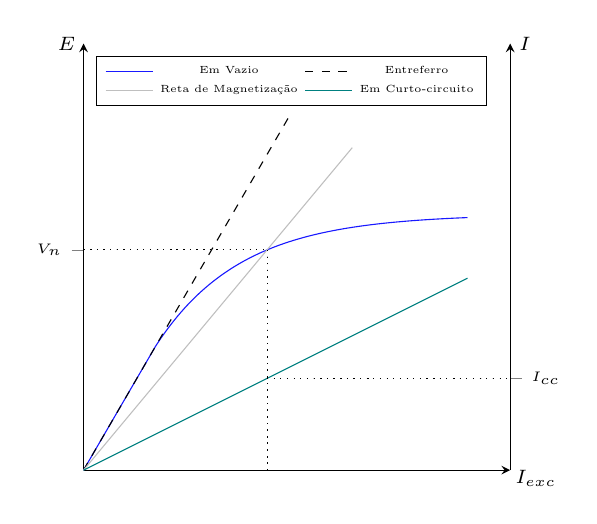
\begin{tikzpicture}
            \begin{axis}[
                xmin=0, xmax=1,
                ymin=0, ymax=2.5,
                axis lines=middle,
                width=7cm,
                height=7cm,
                xtick=\empty, 
                ytick={1.291}, 
                yticklabels={$V_n$},
                tick style={font=\tiny},
                ytick align=outside, 
                xtick align=outside,
                ytick pos=left,
                ticklabel style = {font=\tiny},
                clip=false,
                restrict y to domain=*:2.5,
                legend pos=north west, % Position of the legend
                legend style={
                    legend columns=2,
                    font=\tiny,
                    row sep=0.05pt, % Adjust the vertical spacing between legend entries
                    column sep=1pt, % Adjust the horizontal spacing between legend image and text
                    nodes={scale=0.75, transform shape}
                },
            ]
                \node[font=\scriptsize] at (-0.04,2.5) {$E$};
                \node[font=\scriptsize] at (1.035,2.5) {$I$};
                \node[font=\scriptsize] at (1.06,-0.05) {$I_{exc}$};
        
                % OCC
                \addplot[blue!90, domain=0.1692:0.9, samples=100] ({x},{1.5*(1-1.2*exp(-5*x))});
                \addlegendentry{Em Vazio}
                
                % Entreferro
                \addplot[blue!90, domain=0:0.1692, samples=100, forget plot] ({x},{4.3*x});
                \addplot[dashed, black, domain=0:0.485, samples=100] ({x},{4.3*x});
                \addlegendentry{Entreferro}
        
                % No saturation
                \addplot[gray!50, domain=0:0.63, samples=100] ({x},{3*x});
                \addlegendentry{Reta de Magnetização}
        
                % SC
                \addplot[green!50!blue, domain=0:0.9, samples=100] ({x},{1.25*x});
                \addlegendentry{Em Curto-circuito}
        
                % relevant horizontal values
                \addplot[dotted,black, domain=0:1.291, samples=100] ({0.4302},{x});
                \addplot[dotted,black, domain=0:0.4302, samples=100] ({x},{1.291});
                \addplot[dotted,black, domain=0.4302:1, samples=100] ({x},{0.538});
            \end{axis}
            \begin{axis}[
                xmin=0, xmax=1,
                ymin=0, ymax=2.5,
                axis y line*=right,
                axis x line=none,
                axis lines=left, % Adjusted line
                ytick={0.538}, 
                yticklabels={$I_{cc}$},
                width=7cm,
                height=7cm,
                tick style={font=\tiny},
                ytick align=outside, 
                xtick align=outside,
                ytick pos=right,
                ticklabel style = {font=\tiny},
                clip=false,
                restrict y to domain=*:2.5,
            ]
            \end{axis}
        \end{tikzpicture}
    }
    \caption{Caracteristica em vazio e em curto-circuito}
    \label{fig:maq-sincrona-vazio-e-cc}
\end{figure}
\end{minipage}\hfill
\begin{minipage}[c]{.45\linewidth}
    \begin{mdframed}
        \vspace{2.25cm}
        \hfil (imagem)
        \vspace{2.25cm}
    \end{mdframed}
\end{minipage}

%//==============================--@--==============================//%
\clearpage
\subsubsection{Em Carga}

\noindent A potência nominal de uma máquina síncrona  é a máxima potência aparente à tensão nominal com fp $= 0.85,0.90, 0.95$ que pode fornecer continuamente. O fator que a limita é o aquecimento devido às correntes que percorrem os enrolamentos (limite térmico).

\begin{mdframed}
    \hfil Potência ativa $<$ potência nominal $\rightarrow$ limitada pela potência da máquina de acionamento.
\end{mdframed}

\noindent Quando a máquina está a funcionar à velocidade síncrona e está excitada de modo a apresentar a sua tensão nominal em vazio, podemos assumir que a corrente de carga aumentará gradualmente a partir de zero até atingir o seu valor nominal, mantendo um fator de potência constante.

\begin{minipage}[b]{0.5\linewidth}
   \begin{figure}[H]
        \centering
        \begin{tikzpicture}[>=latex, scale=3]
   
            \coordinate (E) at (0:2.5);
            \coordinate (I) at (-53.13:0.5); 
            \coordinate (I') at (-53.13:1.5);
            \coordinate (V) at (-20:1.791);
            
            % Phasors
            \draw[->,black] (0,0) -- (E) node[right, above] {$E$};
            \draw[->,black] (0,0) -- (I) node[below=-0.01] {$I$};
            \draw[-,gray, dashed] (I) -- (I');
            \draw[->,black] (0,0) -- (V) node[right,below] {$V$};
            \draw[-,gray, dashed] (I') -- (V);
            \draw[->,black] (V) -- (E) node[below=0.15] {$j X_s I$};
        
            % Arcs
            \draw[-] (-20:0.2cm) arc (-20:-53.13:0.2cm) node[yshift=-0.2mm,xshift=2.4mm] {$\phi$};
            \draw[-] (0:0.4cm) arc (0:-20:0.4cm) node[yshift=1.5mm,xshift=2mm] {$\delta$};
            
    \end{tikzpicture}
    \end{figure} 
\end{minipage}\hfill
\begin{minipage}[b]{0.45\linewidth}
    \noindent Do diagrama de fasores, retiramos as seguintes equações:
    $$
    \begin{aligned}
        E \sin(\delta) &= X_s I \cos(\phi)\\
        E \cos(\delta) &= V + X_s I \sin(\phi)
    \end{aligned}
    $$
    Resolvendo em ordem a $V$  e eliminando o ângulo $\delta$, obtem-se:
    
    $$
        \boxed{V = \sqrt{E^2 - X_s^2 I^2 \cos(\phi)^2} - X_s I \sin(\phi)}
    $$
\end{minipage}

\vspace{1em}
\noindent Supondo $E$ constante, \underline{a tensão $V$ vai experimentar variação}:


\hspace{-1.5em}\begin{minipage}[c]{0.45\linewidth}
\noindent Pressupondo uma máquina síncrona com reactância síncrona $X = 1$ p.u. e velocidade nominal constante, com corrente de excitação constante para a tensão nominal em vazio, observamos a variação da tensão nos terminais à medida que a corrente de carga varia de 0 a 1 p.u. para diferentes fatores de potência. \underline{Calculando os extremos}:

\vspace{0.75 em}
\noindent\textbf{Para f.p. = 1:}
$$
    \boxed{V^2 + X_s^2 I^2 = E^2}\; \rightarrow\; \text{Elipse}
$$

\noindent\textbf{Para f.p. = 0:}
$$
    \begin{aligned}
       &\text{Indutivo:}\quad &\boxed{V = E - X_s I}\\
        &\text{Capacitivo:}\quad &\boxed{V = E + X_s I}
    \end{aligned}
$$

\noindent A variação da tensão com a corrente é linear.

\end{minipage}
\begin{minipage}[c]{0.5\linewidth}
\begin{figure}[H]
    \centering
    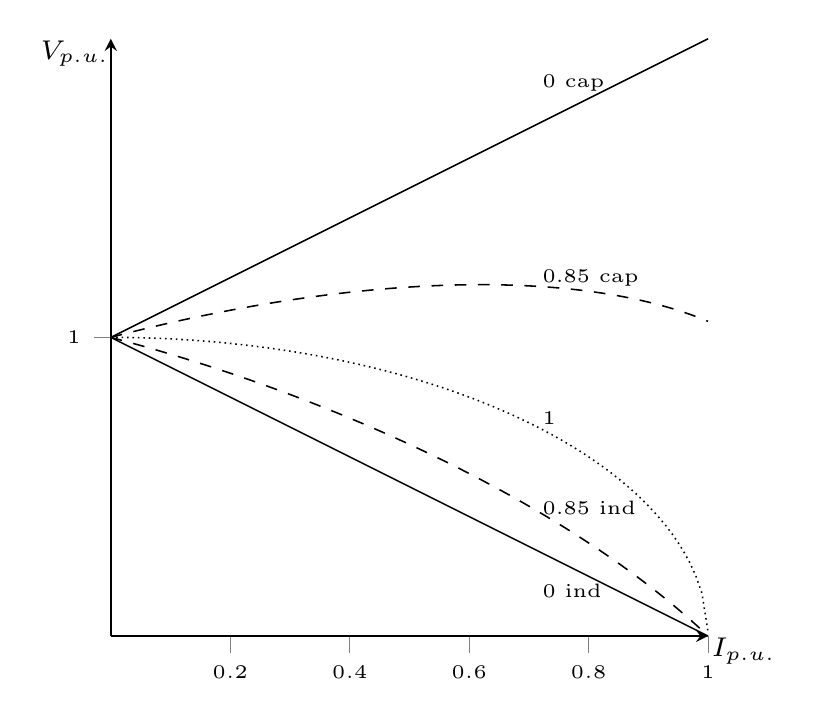
\begin{tikzpicture}[scale=1.4]
        \begin{axis}[
            xmin=0, xmax=1,
            ymin=0, ymax=2,
            axis lines=middle,
            width=7cm,
            height=7cm,
            xtick={0,0.2,0.4,0.6,0.8,1}, 
            ytick={1}, 
            tick style={font=\tiny},
            ytick align=outside, 
            xtick align=outside,
            ytick pos=left,
            ticklabel style = {font=\tiny},
            clip=false
        ]
    
            \node[font=\scriptsize] at (-0.06,1.95) {$V_\text{p.u.}$};
            \node[font=\scriptsize] at (1.06,-0.05) {$I_\text{p.u.}$};
            
             % Plot for delta = 0 ind and cap
            \addplot[black, domain=0:1, samples=100] {1 - x} node[right, font=\tiny] at (axis cs:0.7,0.15) {0 ind};
            \addplot[black, domain=0:1, samples=100] {1 + x} node[right, font=\tiny] at (axis cs:0.7,1.85) {0 cap};
            
            % Plot for delta = 0.85 ind and cap
            \addplot[black,dashed, domain=0:1, samples=100] {sqrt(1 - 0.85^2*x^2) - x*0.52678} node[right, font=\tiny] at (axis cs:0.7,0.43) {0.85 ind};
            \addplot[black,dashed, domain=0:1, samples=100] {sqrt(1 - 0.85^2*x^2) + x*0.52678} node[right, font=\tiny] at (axis cs:0.7,1.2) {0.85 cap};
            
            % Plot for delta = 1
            \addplot[black,densely dotted, domain=0:1, samples=100] {sqrt(1 - x^2)} node[right, font=\tiny] at (axis cs:0.7,0.73) {1};
        \end{axis}
    \end{tikzpicture}
\end{figure} 
\end{minipage}

\vspace{0.5em}
\begin{mdframed}
    \begin{enumerate}
        \item Quando o fator de potência é unitário ou indutivo:
        \begin{itemize}
            \item A tensão diminui à medida que a corrente de carga aumenta.
            \item Isso ocorre devido ao efeito desmagnetizante da reação do induzido, onde o fluxo magnético se subtrai do fluxo principal.
        \end{itemize}
    
        \item Quando o fator de potência é capacitivo:
        \begin{itemize}
            \item A tensão aumenta à medida que a corrente de carga.
            \item Isso ocorre porque a reação do induzido tem um efeito magnetizante, onde o fluxo magnético se soma ao fluxo principal, especialmente em correntes relativamente baixas.
        \end{itemize}
    \end{enumerate}
\end{mdframed}

\clearpage
\noindent Se se pretender  manter constante a tensão então há que \underline{atuar sobre a corrente de excitação que condiciona $E$}. Para uma dada potência ativa, sendo a amplitude de tensão $V$ constante a variação da corrente de excitação altera $E$ donde resulta uma variação de intensidade $I$ e $\sin(\phi)$. A equação anterior pode reescrever-se:

$$
    \boxed{E = \sqrt{V^2 + X_s^2I^2 + 2V X_s I \sin(\phi)}}
$$

\hspace{-1.5em}\begin{minipage}[c]{0.45\linewidth}
\noindent Pressupondo novamente a máquina síncrona com reactância síncrona $X = 1$ p.u. com tensão nominal aos terminais, observamos a variação da f.e.m $E$ à medida que a corrente de carga varia de 0 a 1.0 p.u. para diferentes fatores de potência e potência ativa. \underline{Calculando os extremos}:

\vspace{1 em}
\noindent\textbf{Para P = 0:}
$$
    \boxed{E = V \pm X_s I}\; \rightarrow\; \text{Linear}
$$
$\cos(\phi) = 0$ e consequentemente, $\sin(\phi) = \pm 1$
\noindent\textbf{Para P = 1:}

$$
    \begin{aligned}
            &E = \sqrt{V^2 + X_s^2 I^2}\\
            &\boxed{E^2 - I^2 = 1}\; \rightarrow\; \text{Hiperbole}
    \end{aligned}
$$
$\cos(\phi) = 1$ e consequentemente, $\sin(\phi) = 0$

\vspace{0.5em}
\noindent O fator de potência encontra-se representado a traço interrompido.

\end{minipage}
\begin{minipage}[c]{0.5\linewidth}
\begin{figure}[H]
    \centering
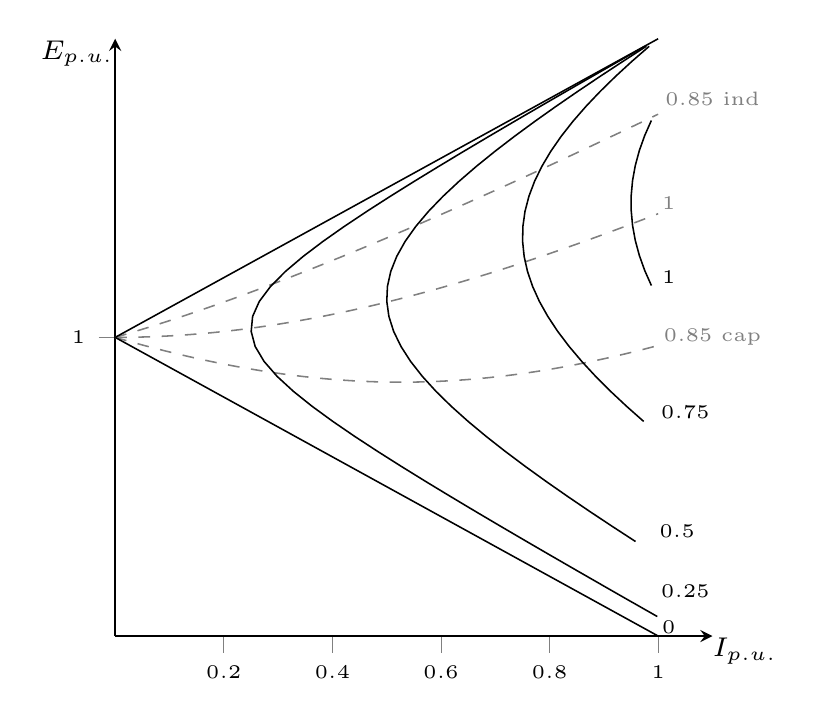
\begin{tikzpicture}[scale=1.4]
    \begin{axis}[
        xmin=0, xmax=1.1,
        ymin=0, ymax=2,
        axis lines=middle,
        width=7cm,
        height=7cm,
        xtick={0,0.2,0.4,0.6,0.8,1}, 
        ytick={1}, 
        tick style={font=\tiny},
        ytick align=outside, 
        xtick align=outside,
        ytick pos=left,
        ticklabel style = {font=\tiny},
        clip=false,
        restrict x to domain=*:1,
    ]

        \node[font=\scriptsize] at (-0.07,1.95) {$E_\text{p.u.}$};
        \node[font=\scriptsize] at (1.16,-0.05) {$I_\text{p.u.}$};

        % Plot for FP = 1
        \addplot [gray,dashed,domain=0:1, samples=100] {sqrt(x^2 + 1)};

        % Plot for FP = 0.85 cap
        \addplot [gray,dashed,domain=0:1, samples=100] {sqrt(x^2 + 2*0.5267*x + 1)};

        % Plot for FP = 0.85 ind
        \addplot [gray,dashed,domain=0:1, samples=100] {sqrt(x^2 - 2*0.5267*x + 1)};
        
         % Plot for P = 0
        \addplot[black, domain=0:1, samples=100] {1 - x};
        \addplot[black, domain=0:1, samples=100] {1 + x};

         % Plot for P = 1
        \addplot [black, samples=200] ({sqrt(x^2 + 1)-0.05},{x+1.45});

        % Plot for P = 0.5
        \addplot [black, samples=200] ({sqrt(x^2 + sqrt(3)*x + 1)},{x + 2});

        % Plot for P = 0.25
       \addplot [black, samples=200] ({sqrt(x^2 + 0.9682*2*x + 1)},{x + 2});

        % Plot for P = 0.75
        \addplot [black, samples=200] ({sqrt(x^2 + 2*0.6613*x + 1)},{x + 2});


        % Lengends
        \node[font=\tiny] at (1.0195,0.03) {$0$};
        \node[font=\tiny] at (1.05,0.15) {$0.25$};
        \node[font=\tiny] at (1.035,0.35) {$0.5$};
        \node[font=\tiny] at (1.05,0.75) {$0.75$};
        \node[font=\tiny] at (1.0195,1.2) {$1$};

        \node[gray, font=\tiny] at (1.1,1) {$0.85$ cap};
        \node[gray, font=\tiny] at (1.1,1.8) {$0.85$ ind};
        \node[gray, font=\tiny] at (1.0195,1.45) {$1$};

    \end{axis}
\end{tikzpicture}
\end{figure} 
\end{minipage}

\vspace{0.5em}
\begin{mdframed}
    \begin{enumerate}
        \item  O valor da corrente te carga é mínimo para f.p $= 1$ (O traço interrompido interceta as curvas hiperbólicas no mínimo relativo ao eixo das abcissas) aumentando à medida que o fator de potência diminui.

        \item Quando traçadas em função da corrente de excitação, estas curvas são conhecidas pela designação de curvas em V. O seu andamento é semelhante ao gráfico da variação da tensão, ainda que não idêntico, por força da saturação da característica em vazio $E(I_\text{exc})$.
    \end{enumerate}
\end{mdframed}

%//==============================--@--==============================//%
\subsubsection{Fórmulas da Potência Ativa e Reativa}

\noindent Tomando a tensão aos terminais de V como referência, a potência complexa fornecida pelo gerador é:

$$
\begin{aligned}
      \mathbf{S}_G = P_G + jQ_G = &\mathbf{V}\mathbf{I}^* = V e^{j 0} e^{j \phi} = VI e^{j \phi}\\
      P_G = V I \cos(\phi)&\qquad
      Q_G = V I \sin(\phi)
\end{aligned}
$$

\noindent Relembrando as expressões do diagrama de fasores, podemos escrever as potências ativa e reativa da seguinte forma:
$$
    \left\{\begin{aligned}
        E \sin(\delta) &= X_s I \cos(\phi)\\
        E \cos(\delta) &= V + X_s I \sin(\phi)
    \end{aligned}\right.\quad
    \rightarrow\quad
    \left\{\begin{aligned}
         P_G &= \frac{E V}{X_s} \sin(\delta)\\
         Q_G &= \frac{V}{X_s} \left(E\cos(\delta) - V\right) =  \frac{V}{X_s} \Delta
    \end{aligned}\right.\qquad
$$

\noindent O ângulo de potência $\delta$ não é uma variável de controlo. Sendo o gerador um conversor mecanoeléctrico, a potência ativa gerada é (à parte as perdas) igual à potência mecânica fornecida pela máquina motriz. Note-se que $\delta$ depende da f.e.m. $E$ e, por conseguinte, da corrente de excitação:

\begin{mdframed}
    \noindent Constata-se que a potência reativa depende da diferença $\Delta$. Admitindo constante a tensão V:
    $$
        \begin{aligned}
            &E \cos(\delta) = V\; \rightarrow\; \text{A potência reativa é controlável através da corrente de excitação que determina a $E$.}\\
            &\mkern140mu \text{A excitação normal é definida para $\delta$ = 0.}\\
            &E \cos(\delta) > V\; \rightarrow\; \text{A máquina fica sobreexcitada e fornece potência reativa.}\\
            &E \cos(\delta) < V\; \rightarrow\; \text{A máquina fica subexcitada e absorve potência reativa.}
        \end{aligned}
    $$
\end{mdframed}

%//==============================--@--==============================//%